\documentclass[UTF8]{ctexart}
\usepackage{amsthm}
\usepackage{amsfonts}
\usepackage{mathrsfs}
\usepackage{graphicx}
\usepackage{geometry}
\usepackage{fancyhdr}
\usepackage{listings}
\usepackage{textcomp}
\usepackage{hyperref}
\usepackage{amsmath,bm}
\renewcommand{\vec}[1]{\boldsymbol{#1}}
\usepackage{amssymb}
\usepackage{verbatim}
\usepackage{enumitem} 
\usepackage{minted}
\usemintedstyle{vs}
\usepackage[framed,numbered,autolinebreaks,useliterate]{mcode}  %For including MATLAB codes, requires file ``mcode.sty" You can use any other packages to include the codes as you like
\lstset{
  breaklines=true, %对过长的代码自动换行
  texcl=true,
  extendedchars=false,columns=flexible,mathescape=true % %设定中文冲突,断行,列模式,数学环境输入,listing数字的样式
}
\lstset{language=Matlab}
\usepackage{hyperref}

\graphicspath{{figures/}} %set the path of inserting figure

% =============================================
% Format setting
% =============================================

\linespread{1.5}
\geometry{top=1in,bottom=1in,left=1in,right=1in}

\newcommand{\cndash}{\rule{0.2em}{0pt}\rule[0.35em]{1.6em}{0.05em}\rule{0.2em}{0pt}} %中文破折号


\begin{document}


%------------中文设置--------------------------
\renewcommand{\refname}{\centerline{参考文献}}
\renewcommand{\tablename}{表}
\renewcommand{\arraystretch}{1.3}
%===================Image settings========================%
\renewcommand{\figurename}{图}
%===============End image settings========================%
%-----------中文设置--------------------------



\pagestyle{fancy}

% =============================================
% Part 1 Edit the information
% =============================================
\renewcommand{\today}{\number\year~年~\number\month~月~\number\day~日}
\fancyhead{}
\lhead{\newtitle}
\chead{姓名:\name}
\rhead{学号:\stuid}
\lfoot{}
\cfoot{第~\thepage~页}
\rfoot{}

\newcommand{\grade}{\hspace{3cm}}
\newcommand{\institute}{智能工程学院}
\newcommand{\major}{智能科学与技术}
\newcommand{\name}{方桂安}
\newcommand{\stuid}{20354027}



\newcommand{\course}{自动驾驶技术基础}
\newcommand{\newtitle}{第 9 周}


\thispagestyle{empty} %%%%Not header and footer in the first page

\begin{figure}[h]
  \begin{minipage}{0.6\linewidth}
    \centerline{\includegraphics[width=\linewidth]{head3.jpg}} %insert the figure of the report's title and school name
  \end{minipage}
  \hfill
  \begin{minipage}{.4\linewidth}
    \raggedleft
    \begin{tabular*}{.8\linewidth}{ll}
      日期: & \underline{\today} \\
      \\
      \\
      成绩: & \underline\grade
    \end{tabular*}
  \end{minipage}
\end{figure}

\begin{table}[!htbp]
  \centering
  \begin{tabular*}{\linewidth}{lll}
    \quad 学院: \underline\institute   &  \quad\quad\quad 课程: \underline\course & \quad\quad\quad 周次:\underline\newtitle  \\
    \quad 专业: \underline\major& \quad\quad\quad 姓名: \underline\name & \quad\quad\quad 学号:  \underline\stuid \\
  \end{tabular*}
\end{table}

% =============================================
% Part 2 Main document
% =============================================

\section{题一}

  \subsection{题目}
  自动驾驶为了出色地完成驾驶任务,可分为哪四大模块?
  \subsection{解答}
  %无序列表
  \begin{itemize}
    \item 感知系统
    \item 地图和定位
    \item 决策与规划
    \item 控制与建模
  \end{itemize}

\section{题二}

  \subsection{题目}
  系统建模一般分哪两种建模方式?
  \subsection{解答}
  \par (1)\textbf{机理建模}

  根据系统的运动学或动力学的规律和机理,如机械系统中的牛顿定律、电系统中的基尔霍夫定律等,建立系统的数学表达式。要求已知所有元部件的结构及对应的物理机理。
  \par (2)\textbf{实验建模}

  人为地给系统施加某种典型的输入信号,记录下对应的输出响应数据,通过辨识的方法采用适当的数学模型去模拟逼近该过程,所获得的数学模型称为辨识模型。

\section{题三}

  \subsection{题目}
  请写出高速转向车辆模型的简化横向误差模型(即四个状态为误差)
  \subsection{解答}
  $$
\begin{aligned}
&\delta \rightarrow 0 \\
&\Rightarrow \alpha_{f} \rightarrow 0, \alpha_{r} \rightarrow 0, v_{x} \gg v_{y} \\
&{\left[\begin{array}{c}
\dot{X} \\
\dot{Y} \\
\dot{\psi} \\
\dot{v}_{x} \\
\dot{v}_{y} \\
\dot{\omega}
\end{array}\right]=\left[\begin{array}{c}
v_{x} \cos \psi-v_{y} \sin \psi \\
v_{y} \cos \psi+v_{x} \sin \psi \\
\omega \\
\frac{1}{m}\left(F_{x r}+\cos \delta F_{x f}-\sin \delta F_{y f}+m v_{y} \omega\right) \\
\frac{1}{m}\left(F_{y r}+\sin \delta F_{x f}+\cos \delta F_{y f}-m v_{x} \omega\right) \\
\frac{1}{I_{z}}\left(l_{f} F_{x f} \sin \delta+l_{f} F_{y f} \cos \delta-F_{y r} l_{r}\right)
\end{array}\right] \approx\left[\begin{array}{c}
v_{x} \cos \psi-v_{y} \sin \psi \\
v_{y} \cos \psi+v_{x} \sin \psi \\
\omega \\
\frac{1}{m}\left(F_{x r}+F_{x f}\right) \\
\frac{1}{m}\left(F_{y r}+F_{y f}-m v_{x} \omega\right) \\
\frac{1}{I_{z}}\left(l_{f} F_{y f}-F_{y r} l_{r}\right)
\end{array}\right]}
\end{aligned}
$$
$$
\begin{aligned}
&\alpha_{r}=\frac{v_{y}-l_{r} \omega}{v_{x}} \\
&\alpha_{f}=-\delta+\frac{v_{y}+l_{f} \omega}{v_{x}} \\
&F_{y r}=-2 K_{r} \alpha_{r} \\
&F_{y f}=-2 K_{f} \alpha_{f} \\
&F_{x r}=\left(C_{m 1}-C_{m 2} v_{x}\right) d-C_{r} N-C_{d} v_{x}^{2} \\
&F_{x f}=-C_{r} N-C_{d} v_{x}^{2}
\end{aligned}
$$
则横向加速度误差
$$
\ddot{e}_{1}=a_{y}-a_{y d e s}=\left(\dot{v}_{y}+v_{x} \dot{\psi}\right)-v_{x} \dot{\psi}_{d e s}=\dot{v}_{y}+v_{x}\left(\dot{\psi}-\dot{\psi}_{d e s}\right)=\dot{v}_{y}+v_{x}\left(\omega-\omega_{d e s}\right)
$$
横向速度误差~~~$\quad \dot{e}_{1}=v_{y}+v_{x}\left(\psi-\psi_{d e s}\right)$\\
航向误差~~~$e_{2}=\psi-\psi_{\text {des }}$\\
航向角速度误差~~~$\quad \dot{e}_{2}=\dot{\psi}-\dot{\psi}_{d e s}=\omega-\omega_{d e s}$\\
航行角加速度误差~~~$\quad \ddot{e}_{2}=\dot{\omega}-\dot{\omega}_{\text {des }}$
 
\begin{figure*}[h] 
  \centering
  \left[\begin{array}{c}
    \dot{e}_{1} \\
    \ddot{e}_{1} \\
    \dot{e}_{2} \\
    \ddot{e}_{2}
    \end{array}\right]=\left[\begin{array}{cccc}
    0 & 1 & 0 & 0 \\
    0 & -\frac{2 K_{r}+2 K_{f}}{m v_{x}} & \frac{2 K_{r}+2 K_{f}}{m} & -\frac{2 l_{f} K_{f}-2 l_{r} K_{r}}{m v_{x}} \\
    0 & 0 & 0 & 1 \\
    0 & -\frac{2 l_{f} K_{f}-2 l_{r} K_{r}}{I_{z} v_{x}} & \frac{2 l_{f} K_{f}-2 l_{r} K_{r}}{I_{z}} & -\frac{2 l_{f}^{2} K_{f}+2 l_{r}^{2} K_{r}}{I_{z} v_{x}}
    \end{array}\right]
    \left[\begin{array}{c}
      e_{1} \\
      \dot{e}_{1} \\
      e_{2} \\
      \dot{e}_{2}
      \end{array}\right]+\left[\begin{array}{c}
      0 \\
      \frac{2 K_{f}}{m} \\
      0 \\
      \frac{2 l_{f} K_{f}}{I_{z}}
      \end{array}\right] \delta+\left[\begin{array}{c}
      0 \\
      -\frac{2 l_{f} K_{f}-2 l_{r} K_{r}}{m v_{x}}-v_{x} \\
      0 \\
      -\frac{2 l_{f}^{2} K_{f}+2 l_{r}^{2} K_{r}}{I_{z} v_{x}}
      \end{array}\right] \omega_{\text {des }}+\left[\begin{array}{c}
      0 \\
      0 \\
      0 \\
      -1
      \end{array}\right] \dot{\omega}_{\text {des }}

\end{figure*}



\section{题四}

  \subsection{题目}
  二次型性能指标函数一般包含哪三项优化项?
  \subsection{解答}
  \par (1) 积分项 $\frac{1}{2} \int_{t_{0}}^{t_{f}} e^{\mathrm{T}}(t) Q(t) e(t) \mathrm{d} t$
  
  设积分项
  $$
  L_{e}=\frac{1}{2}\left[e^{\mathrm{T}}(t) \boldsymbol{Q}(t) e(t)\right]=\frac{1}{2} \sum_{i=1}^{m} \sum_{j=1}^{m} q_{i j}(t) e_{i}(t) e_{j}(t)
  $$
  由于 $\boldsymbol{Q}(t)$ 为半正定, 在 $\left[t_{0}, t_{f}\right]$ 非负, 积分 $\int_{t_{0}}^{t_{e}} L_{e} \mathrm{~d} t$ 表示了在区间上误差大小, 反映了 系统在控制过程中动态跟踪误差的累积和。由于误差的二次型表达形式, 所以权矩阵 $\boldsymbol{Q}(t)$ 实际上能给较大的误差以较大的加权, 而 $Q(t)$ 为时间函数, 则意味着对不同时刻误差赋 予不同的加权, 该项反映了系统的控制效果。
  \par (2) 积分项 $\frac{1}{2} \int_{t_{0}}^{t_{f}} u^{\top}(t) R(t) u(t) \mathrm{d} t$
  
  设积分项
  $$
  L_{u}=\frac{1}{2}\left[\boldsymbol{u}^{\mathrm{T}}(t) \boldsymbol{R}(t) \boldsymbol{u}(t)\right]=\frac{1}{2} \sum_{i=1}^{r} \sum_{j=1}^{r} r_{i j}(t) u_{i}(t) u_{j}(t)
  $$
  由于 $\boldsymbol{R}(t)>0$, 且对称, 而控制信号的大小往往正比于作用力或力矩, 故 $\int_{t_{0}}^{t_{f}} L_{u} \mathrm{~d} t$ 表 示了在整个控制过程中所消耗的控制能量。 $\boldsymbol{R}(t)$ 实际上能给各控制分量赋予不同的权, 它是时间的函数,则意味着对不同时刻的控制分量赋子不同的加权。
  \par (3) 终值项 $\frac{1}{2} e^{\mathrm{T}}\left(t_{f}\right) \boldsymbol{F e}\left(t_{f}\right)$
  
  设终值项
  $$
  \frac{1}{2} \boldsymbol{e}^{\mathrm{T}}\left(t_{j}\right) \boldsymbol{F e}\left(t_{f}\right)=\frac{1}{2} \sum_{i=1}^{m} \sum_{j=1}^{m} f_{i j} e_{i}(t) e_{j}(t)
  $$
  终值项的物理含义是表示在控制过程结束后, 对系统终态跟踪误差的要求, 强调了 系统接近终端时的误差。该项也同样反映了系统的控制要求。如对终端误差限制为 $e\left(t_{f}\right)=0$, 此项可略去。
  
  综上所述, 使二次型性能指标式极小的物理意义是:使系统在整个控制过程中的动态跟踪误差与控制能量消耗, 以及控制过程结束时的终端跟踪误差综合最优。

\section{题五}

  \subsection{题目}
  线性二次问题三种重要形式分别是?
  \subsection{解答}
  \par (1)\textbf{状态调节器}:
  $$
  \begin{aligned}
  &\dot{\boldsymbol{x}}(t)=\boldsymbol{A}(t) \boldsymbol{x}(t)+\boldsymbol{B}(t) \boldsymbol{u}(t), \quad \boldsymbol{x}\left(t_{0}\right)=\boldsymbol{x}_{0} \\
  &\boldsymbol{y}(t)=\boldsymbol{C}(t) \boldsymbol{x}(t) \\
  &\boldsymbol{C}(t)=I, \boldsymbol{y}_{r}(t)=0 \\
  &\Rightarrow \boldsymbol{e}(t)=-\boldsymbol{y}(t), \boldsymbol{y}(t)=\boldsymbol{x}(t)
  \end{aligned}
  $$
  二次型性能指标:
  $$
  \begin{aligned}
  &J=\frac{1}{2} \boldsymbol{e}^{T}\left(t_{f}\right) \boldsymbol{F e}\left(t_{f}\right)+\frac{1}{2} \int_{t_{0}}^{t_{f}} \boldsymbol{e}^{T}(t) \boldsymbol{Q}(t) \boldsymbol{e}(t)+\boldsymbol{u}^{T}(t) \boldsymbol{R}(t) \boldsymbol{u}(t) d t \\
  &=\frac{1}{2} \boldsymbol{x}^{T}\left(t_{f}\right) \boldsymbol{F} \boldsymbol{x}\left(t_{f}\right)+\frac{1}{2} \int_{t_{0}}^{t_{f}} \boldsymbol{x}^{T}(t) \boldsymbol{Q}(t) \boldsymbol{x}(t)+\boldsymbol{u}^{T}(t) \boldsymbol{R}(t) \boldsymbol{u}(t) d t
  \end{aligned}
  $$
  $\boldsymbol{F}$ 为半正定 $m \times m$ 常数矩阵; $\boldsymbol{Q}(t)$ 为半正定 $m \times m$ 对称矩阵; $\boldsymbol{R}(t)$ 为正定 $r \times r$ 对称矩阵; 终端时刻 $t_{f}$ 固定。
  
  这时,线性二次型最优控制问题为,当系统受扰偏离原零平衡状态时,要求产 生一控制向量, 使系统状态 $x(t)$ 恢复到原平衡状态附近, 并使性能指标极小。 因而, 称为状态调节器问题。
  \par (2)\textbf{输出调节器}: 
  
  $$
  \begin{aligned}
  &\dot{\boldsymbol{x}}(t)=\boldsymbol{A}(t) \boldsymbol{x}(t)+\boldsymbol{B}(t) \boldsymbol{u}(t), \quad \boldsymbol{x}\left(t_{0}\right)=\boldsymbol{x}_{0}\\
  &\boldsymbol{y}(t)=\boldsymbol{C}(t) \boldsymbol{x}(t) \\
  &\boldsymbol{y}_{r}(t)=0 \Rightarrow \boldsymbol{e}(t)=-\boldsymbol{y}(t)
  \end{aligned}
  $$
  二次型性能指标:
  $$
  \begin{aligned}
  &J=\frac{1}{2} \boldsymbol{e}^{T}\left(t_{f}\right) \boldsymbol{F e}\left(t_{f}\right)+\frac{1}{2} \int_{t_{0}}^{t_{f}} \boldsymbol{e}^{T}(t) \boldsymbol{Q}(t) \boldsymbol{e}(t)+\boldsymbol{u}^{T}(t) \boldsymbol{R}(t) \boldsymbol{u}(t) d t \\
  &=\frac{1}{2} \boldsymbol{y}^{T}\left(t_{f}\right) \boldsymbol{F} \boldsymbol{y}\left(t_{f}\right)+\frac{1}{2} \int_{t_{0}}^{t_{f}} \boldsymbol{y}^{T}(t) \boldsymbol{Q}(t) \boldsymbol{y}(t)+\boldsymbol{u}^{T}(t) \boldsymbol{R}(t) \boldsymbol{u}(t) d t
  \end{aligned}
  $$
  $\boldsymbol{F}$ 为半正定 $m \times m$ 常数矩阵; $\boldsymbol{Q}(t)$ 为半正定 $m \times m$ 对称矩阵; $\boldsymbol{R}(t)$ 为正定 $r \times r$ 对称矩阵; 终端时刻 $t_{f}$ 固定。
  
  这时线性二次型最优控制问题为:当系统受扰偏离原输出平衡状态时,要求产生 一控制向量, 使系统输出 $y(t)$ 保持在原平衡状态附近, 并使性能指标极小, 因而 称为输出调节器。
  \par (3)\textbf{输出跟踪器}:
  $$\quad \begin{aligned} \dot{\boldsymbol{x}}(t) &=\boldsymbol{A}(t) \boldsymbol{x}(t)+\boldsymbol{B}(t) \boldsymbol{u}(t), \quad \boldsymbol{x}\left(t_{0}\right)=\boldsymbol{x}_{0} \\ \boldsymbol{y}(t) &=\boldsymbol{C}(t) \boldsymbol{x}(t) \end{aligned}$$
  二次型性能指标: $$\quad J=\frac{1}{2} \boldsymbol{e}^{T}\left(t_{f}\right) \boldsymbol{F e}\left(t_{f}\right)+\frac{1}{2} \int_{t_{0}}^{t_{f}} \boldsymbol{e}^{T}(t) \boldsymbol{Q}(t) \boldsymbol{e}(t)+\boldsymbol{u}^{T}(t) \boldsymbol{R}(t) \boldsymbol{u}(t) d t \quad $$
  $\boldsymbol{F}$ 为半正定 $m \times m$ 常数矩阵; $\boldsymbol{Q}(t)$ 为半正定 $m \times m$ 对称矩阵; $\boldsymbol{R}(t)$ 为正定 $r \times r$ 对称矩阵; 终端时刻 $t_{f}$ 固定。
  
  针对线性系统状态空间表达式和二次型性能指标式, 当 $\boldsymbol{C}(t) \neq \boldsymbol{I}, \boldsymbol{y}_{\boldsymbol{r}}(t) \neq 0$ 时, 线性二次型最优控制问题归结为: 当理想输出向量 $y_{r}(t)$ 作用于系统时, 要求系 统产生一控制向量, 使系统实际输出向量 $\boldsymbol{y}(t)$ 始终跟踪 $y_{r}(t)$ 的变化, 并使性能指标 式极小。也就是说以极小的控制能量为代价, 使误差保持在零值附近。因而, 这一类线性二次型最优控制问题称为输出跟踪器问题。

\section{题六}

  \subsection{题目}
  Kalman Filter(LQE)如何通过LQR求得,请写出matlab关键代码,即:xxx=lqr(xxx) 。
  \subsection{解答}
  $$
  \because
    \begin{aligned}
      &L^{T}=\operatorname{lqr}\left(A^{T}, C^{T}, R_{w w}, R_{v v}\right) \\
      &L=\operatorname{lqe}\left(A, G, C, R_{w w}, R_{v v}\right)
    \end{aligned}
  $$
  \lstinputlisting[language=Matlab]{code/kf.m}

\section{编程实践题}
%插入图片
\begin{figure}[h]
\centering
\includegraphics[width=0.8\textwidth]{figures/kf.jpg}
\end{figure}

  \subsection{题目}
  给定一个双质系统: $m_{1}=2, m_{2}=1$, 弹簧系数 $k=5$, 阻尼 $\sigma=0.1$, 质量块与地面的滑动阻尼 $\delta=0.1$ (与速度有成正比)。初始时刻 $m_{1}$ 质量块处于 $\mathrm{x}=0$ 的位置, 两质量块距离为 0 。现在 $m_{2}$ 处作用一外力 $F$ 拖动系统使 $m_{1}$ 与 $m_{2}$ 质量块均处于 $x=5$ 的位置。
  \subsection{解答}
  \subsubsection{对系统建模(系统可以直接测量两个物体的位置)}
  \par 考虑系统的状态空间表达式:
  %状态空间表达式
  $$
  \left\{\begin{array}{l}
    \dot{x}=A x+B u+w \\
    y=C x+\nu
    \end{array}\right.
  $$
  
  其中,$A$ 为状态空间表达式的系数矩阵, $B$ 为系统的输入矩阵, $C$ 为系统的输出矩阵, $w$ 为系统的状态噪声, $u$ 为系统的输入, $x$ 为系统的状态, $y$ 为系统的输出, $\nu$ 为系统的输出噪声。且噪声的均值为0并满足高斯分布。
  
  根据题意, 取两质量块的初始位置为坐标系原点, 外力 $F$ 方向 (向右) 为正方向。选择质量块 $m_{1}$ 、 $m_{2}$ 的速度 $\dot{x}_{1} 、 \dot{x}_{2}$,位移 (位置) $x_{1} 、 x_{2}$ 作为状态变量。即状态向量 $\boldsymbol{x}=\left[\dot{x}_{1} \quad \dot{x}_{2} \quad x_{1} \quad x_{2}\right]^{\mathrm{T}}$ 。设控制 变量 $u=F$ 。
  %插入图片
  \begin{figure}[h]
  \centering
  \includegraphics[width=0.8\textwidth]{figures/force.jpg}
  \caption{质量块受力图}
  \label{fig:force}
  \end{figure}

  质量块$m_1,m_2$的受力情况如图\ref{fig:force}所示。
  对每一个质量块应用牛顿运动定律, 可得系统的运动方程。对于 $m_{1}$, 有
  $$
  m_{1} \ddot{x}_{1}=k\left(x_{2}-x_{1}\right)+\sigma\left(\dot{x}_{2}-\dot{x}_{1}\right)-\delta \dot{x}_{1}
  $$
  对于 $m_{2}$, 有
  $$
  m_{2} \ddot{x}_{2}=F-k\left(x_{2}-x_{1}\right)-\sigma\left(\dot{x}_{2}-\dot{x}_{1}\right)-\delta \dot{x}_{2}
  $$
  整理上述两式可得
  $$
  \begin{aligned}
  \ddot{x}_{1} &=-\frac{1}{m_{1}}(\delta+\sigma) \dot{x}_{1}+\frac{\sigma}{m_{1}} \dot{x}_{2}-\frac{k}{m_{1}} x_{1}+\frac{k}{m_{1}} x_{2} \\
  \ddot{x}_{2} &=\frac{\sigma}{m_{2}} \dot{x}_{1}-\frac{1}{m_{2}}(\delta+\sigma) \dot{x}_{2}+\frac{k}{m_{2}} x_{1}-\frac{k}{m_{2}} x_{2}+\frac{F}{m_{2}} \\
  \dot{x}_{1} &=\dot{x}_{1} \\
  \dot{x}_{2} &=\dot{x}_{2}
  \end{aligned}
  $$
  将此微分方程组化为向量矩阵形式, 即得系统状态方程为
$$
\left[\begin{array}{c}
\ddot{x}_{1} \\
\ddot{x}_{2} \\
\dot{x}_{1} \\
\dot{x}_{2}
\end{array}\right]=\left[\begin{array}{cccc}
-\frac{1}{m_{1}}(\delta+\sigma) & \frac{\sigma}{m_{1}} & -\frac{k}{m_{1}} & \frac{k}{m_{1}} \\
\frac{\sigma}{m_{2}} & -\frac{1}{m_{2}}(\delta+\sigma) & \frac{k}{m_{2}} & -\frac{k}{m_{2}} \\
1 & 0 & 0 & 0 \\
0 & 1 & 0 & 0
\end{array}\right]\left[\begin{array}{c}
\dot{x}_{1} \\
\dot{x}_{2} \\
x_{1} \\
x_{2}
\end{array}\right]+\left[\begin{array}{c}
0 \\
\frac{1}{m_{2}} \\
0 \\
0
\end{array}\right] F
$$
因此,
$$
\boldsymbol{A}=\left[\begin{array}{cccc}
-\frac{1}{m_{1}}(\delta+\sigma) & \frac{\sigma}{m_{1}} & -\frac{k}{m_{1}} & \frac{k}{m_{1}} \\
\frac{\sigma}{m_{2}} & -\frac{1}{m_{2}}(\delta+\sigma) & \frac{k}{m_{2}} & -\frac{k}{m_{2}} \\
1 & 0 & 0 & 0 \\
0 & 1 & 0 & 0
\end{array}\right], \quad \boldsymbol{B}=\left[\begin{array}{c}
0 \\
\frac{1}{m_{2}} \\
0 \\
0
\end{array}\right]
$$
由于系统可以直接测量两个物体的位置,故$ C = \left[
  \begin{array}{llll}
    0 & 0 & 1 & 0 \\
    0 & 0 & 0 & 1 
  \end{array}\right] $

考虑性能指标为
$$
J=\frac{1}{2} \int_{0}^{\infty}\left[\boldsymbol{y}^{\mathrm{T}} \boldsymbol{Q} \boldsymbol{y}+\boldsymbol{u}^{\mathrm{T}}(t) \boldsymbol{R} \boldsymbol{u}(t)\right] d t
$$
其中取,
$$
\boldsymbol{Q}=\left[\begin{array}{llll}
2 & 0 & 0 & 0 \\
0 & 2 & 0 & 0 \\
0 & 0 & 1 & 0 \\
0 & 0 & 0 & 1
\end{array}\right], \quad \boldsymbol{R}=1
$$
  \subsubsection{判断系统可控性与可观性}
  \par (1)\textbf{判断可控性}。
系统状态可控的充分必要条件是其能控性矩阵 $\boldsymbol{Q}_{k}=\left[\begin{array}{lllll}\boldsymbol{B} & \boldsymbol{A} \boldsymbol{B} & \boldsymbol{A}^{2} \boldsymbol{B} & \cdots & \boldsymbol{A}^{n-1} \boldsymbol{B}\end{array}\right]$ 满秩, 即 $\operatorname{rank} \boldsymbol{Q}_{k}=n, n$ 为系统的阶次。本系统 $n=4$, 由 MATLAB 计算 $\operatorname{rank}\left[\boldsymbol{B} \quad \boldsymbol{A} \boldsymbol{B} \quad \boldsymbol{A}^{2} \boldsymbol{B} \quad \boldsymbol{A}^{3} \boldsymbol{B}\right]=4$, 因此该系统具有能控性。
  \par (2) \textbf{判断可观性}。
系统状态可观的充分必要条件是其能观测性矩阵 $\boldsymbol{Q}_{g}=\left[\begin{array}{lllll}\boldsymbol{C} & \boldsymbol{C A} & \boldsymbol{C} \boldsymbol{A}^{2} & \cdots & \boldsymbol{C} \boldsymbol{A}^{n-1}\end{array}\right]$ 满秩, 即 $\mathrm{rank} \boldsymbol{Q}_{g}=$ $n$ 。本系统 $n=4$, 由 MATLAB 计算 $\operatorname{rank}\left[\boldsymbol{C} \quad \boldsymbol{C A} \quad \boldsymbol{C A}^{2} \quad \boldsymbol{C A}^{3}\right]=4$, 因此该系统具有能观测性。
  \subsubsection{设计实现LQG控制器并绘制闭环控制性能曲线}
  \begin{figure}
  \centering
  \includegraphics[width=0.8\textwidth]{figures/simulink.png}
  \end{figure}
详细代码见附录,由此可绘制以下闭环控制性能曲线。
\begin{figure}
\centering
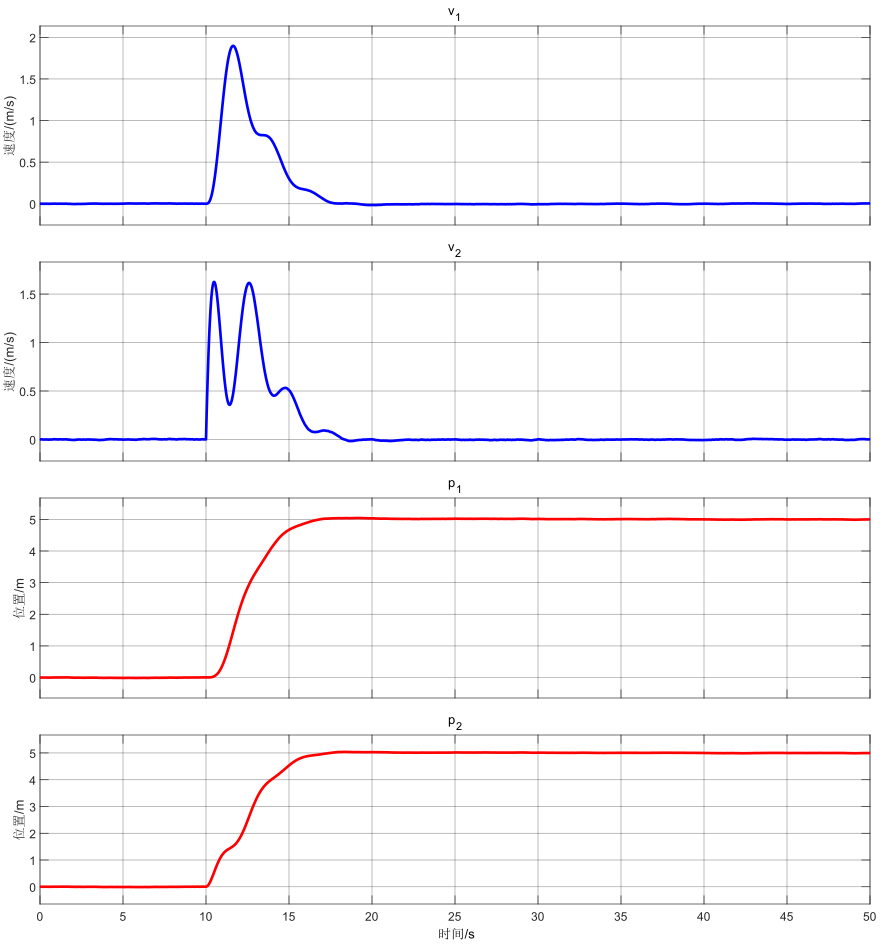
\includegraphics[width=0.8\textwidth]{figures/result.jpg}
\caption{状态变量变化图}
\end{figure}
\begin{figure}
  \centering
  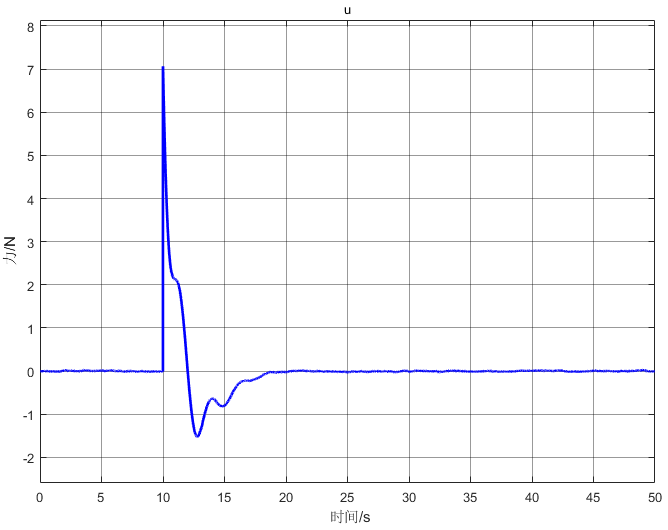
\includegraphics[width=0.8\textwidth]{figures/result2.jpg}
  \caption{外力变化图}
  \label{fig:force}
  \end{figure}

$ v_1,p_1 $是质量块$ m_1 $的速度与位置,$ v_2,p_2 $是质量块$ m_2 $的速度与位置,
由图\ref{fig:force}可知,在t=10s开始施加外力,大约在t=20s时系统趋于稳定,两
质量块从原点移动到p=5m的位置。

\newpage
\appendix
\vspace{.5in}
\section{附录:代码}
\lstinputlisting[language=Matlab]{code/hw_lqg.m}

\end{document}
